\documentclass[11pt]{article}            % Report class in 11 points
\parindent0pt  \parskip10pt             % make block paragraphs
\usepackage{graphicx}
\usepackage{listings}
\newcommand\tab[1][1cm]{\hspace*{#1}}
\usepackage{float}
\usepackage[document]{ragged2e}
\graphicspath{ {images/} }
\usepackage{graphicx} %  graphics header file
\begin{document}
\begin{titlepage}
    \centering
  \vfill
    
\includegraphics[width=8cm]{uni_logo.png} \\ 
	\vskip2cm
    {\bfseries\Large
	Data Structure and Algorithm \\ (CS09203)\\
	
	\vskip2cm
	Lab Report 
	 
	\vskip2cm
	}    

\begin{center}
\begin{tabular}{ l l  } 

Name: & Muhammad Umer \\ 
Registration \#: & CSU-F16-104 \\ 
Lab Report \#: & 01 \\ 
 Dated:& 26-03-2018\\ 
Submitted To:& Mr. Usman Ahmed\\ 

 %\hline
\end{tabular}
\end{center}
    \vfill
    The University of Lahore, Islamabad Campus\\
Department of Computer Science \& Information Technology
\end{titlepage}


    
    {\bfseries\Large
\centering
	Experiment \# 3 \\

Stack with Array implementation\\
	
	}    
 \vskip1cm
 \textbf {Objective}\\ The objective of this session is to understand the various operations on stack using arrays structure in C++.\\~\\
 \textbf {Software Tool} \\
1.  Window 7 (32-bit)\\
2. Sublime Text Editor\\
3. Dev C++

\textbf{Theory:-}\\
Stacks are the most important in data structures. The notation of a stack in computer science is the
same as the notion of the Stack to which you are accustomed in everyday life. For example, a
recursion program on which function call itself, but what happen when a function which is calling
itself call another function. Such as a function ‘A’ call function ‘B’ as a recursion. So, the firstly
function ‘B’ is call in ‘A’ and then function ‘A’ is work. So, this is a Stack. This is a Stack is First
in Last Out data structure.\\~\\

\textbf{Insertions in Stack:}\\
In Stacks, we know the array work, sometimes we need to modify it or add some element in it. For
that purpose, we use insertion scheme. By the use of this scheme we insert any element in Stacks
using array. In Stack, we maintain only one node which is called TOP. And Push terminology is
used as insertions.\\~\\

\textbf{Deletion in Stack:}\\
In the deletion process, the element of the Stack is deleted on the same node which is called TOP.
In stacks, it’s just deleting the index of the TOP element which is added at last. In Stacks Pop
terminology is used as deletion.\\~\\

\textbf{Display of Stack:}\\
In displaying section, the elements of Stacks are being display by using loops and variables as a
reverse order. Such that, last element is display at on first and first element enters display at on
last.\\~\\


\textbf{Algorithm for top of stack varying method:-}\\~\\
\begin{lstlisting}[language=C++]
1. Declare and initialize necessary variables, eg top = -1, MAXSIZE etc.
2. For push operation, if top = MAXSIZE - 1
print "stack overflow"
else
top = top + 1;
 Read item from user
stack[top] = item
3. For next push operation, goto step 2.
4. For pop operation,
If top = -1
 print "Stack underflow"
Else
 item = stack[top]
 top = top - 1
 Display item
5. For next pop operation, goto step 4.
6. Stop
\end{lstlisting}

\textbf{Lab Task:-}\\
1. Insertion in stack\\
2. Deletion in stack\\
3. Display the stack\\~\\


\textbf{Solution:-}\\~\\
\begin{lstlisting}[language=C++]
#include<iostream>
#include<conio.h>
#define SIZE 101
using namespace std;
int stack[SIZE];
int top = -1;

void push(){
	if(top == SIZE-1){
		cout<<"\n\nError: Stack Overflow!";
		cout<<"\n\nPress any key to continue....";
		getch();
		return;
	}
	else
		top++;
	int item;
	cout<<"\n\nEnter value to insert: ";
	cin>>item;
	stack[top] = item;
	cout<<"\n\nValue inserted Successfully";
	cout<<"\n\nPress any key to continue....";
	getch();
}

void pop(){
	int item;
	if(top == -1){
		cout<<"\n\nError: Stack Underflow!";
		cout<<"\n\nPress any key to continue....";
		getch();
		return;
	}
	else{
		item = stack[top];
		top--;
		cout<<"\n\n"<<item<<" is removed from stack!";
	}
	cout<<"\n\nPress any key to continue....";
	getch();
}

void display(){
	if(top == -1){
		cout<<"\n\nError: Stack is Empty!";
		cout<<"\n\nPress any key to continue....";
		getch();
		return;
	}
	cout<<"\n\nItems in stack\n\n";
	for(int i=0; i<=top; i++){
		cout<<stack[i]<<" ";
	}
	cout<<"\n\nPress any key to continue....";
	getch();
}

int main(){
	int choice;
	up:
	system("cls");
	cout<<"\t\t\tMAIN MENU\n\n";
	cout<<"\tPRESS\n\n";
	cout<<"\t1 FOR INSERTION\n\n";
	cout<<"\t2 FOR DELETION\n\n";
	cout<<"\t3 FOR DISPLAY\n\n";
	cout<<"\t4 TO EXIT\n\n";
	cout<<"PLEASE ENTER YOUR CHOICE\n\n";
	cin>>choice;
	if(choice == 1){
		push();
		goto up;
	}
	else if(choice == 2){
		pop();
		goto up;
	}
	else if(choice == 3){
		display();
		goto up;
	}
	else if(choice == 4)
		exit(0);
	else{
		cout<<"\n\nWRONG CHOICE!";
		cout<<"\n\nPRESS ANY KEY TO CHOOSE AGAIN...";
		getch();
		goto up;
	}
	return 0;
}
\end{lstlisting}

\textbf{Output:-}
\begin{figure}[H]
\centering
  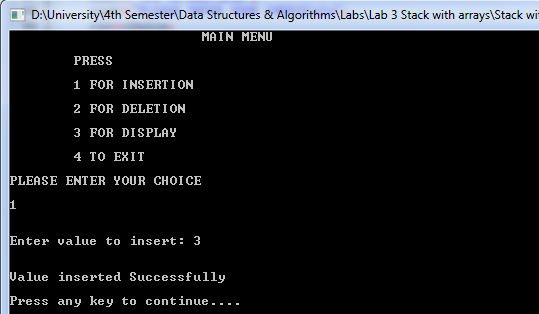
\includegraphics[width=12cm,height=6cm,keepaspectratio]{1.png}
\caption{Main menu and insertion operation}
\label{Figure:3}    
\end{figure}

\begin{figure}[H]
\centering
  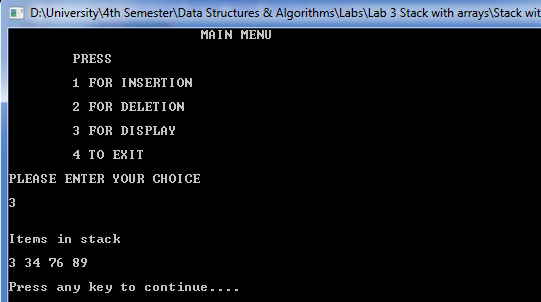
\includegraphics[width=12cm,height=6cm,keepaspectratio]{2.png}
\caption{Displaying after insertion}
\label{Figure:4}    
\end{figure}

\begin{figure}[H]
\centering
  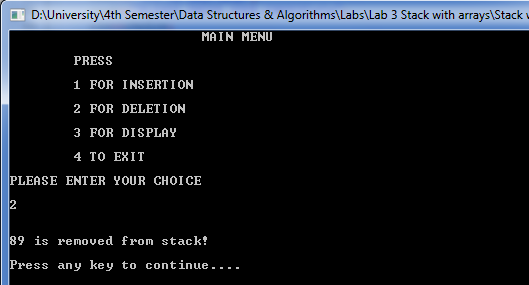
\includegraphics[width=12cm,height=6cm,keepaspectratio]{3.png}
\caption{Deleting operation}
\label{Figure:5}    
\end{figure}

\begin{figure}[H]
\centering
  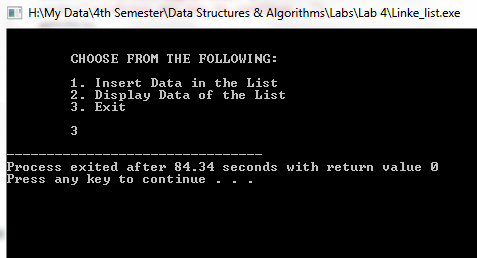
\includegraphics[width=12cm,height=6cm,keepaspectratio]{4.png}
\caption{Displaying after deletion}
\label{Figure:6}    
\end{figure}

\begin{figure}[H]
\centering
  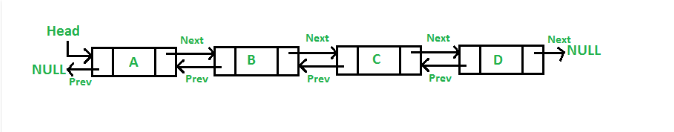
\includegraphics[width=12cm,height=6cm,keepaspectratio]{5.png}
\caption{Exit}
\label{Figure:7}    
\end{figure}

\textbf{Source Code:-}
https://github.com/umerayan/Data-Structure-and-Algorithms\\~\\

\textbf{Conclusion:-}
Statck in Data Structure work as First in Last out (FILO) concept. Stacks are the most important in data structures. Recursive function is one of the best example of stack. In this lab we implemented program for stack which is given above.
The program is written in C++ and open source for everyone at my github account (The link provided above).\\~\\~\\

\tab[6cm] \noindent\rule{6cm}{0.4pt}\\
\tab[6cm] (Concerned Teacher/Lab Engineer)
 
\end{document}                          % The required last line
